\documentclass[17pt]{beamer}
\usetheme{Warsaw}
\useoutertheme{infolines}
\usepackage[utf8]{inputenc}
\usepackage{t1enc}
\usepackage[magyar]{babel}
\usepackage{graphicx}
\usepackage{amsmath}
\usepackage{array}
\setbeamercovered{dynamic}
\frenchspacing
\usepackage{colortbl}

\title{QR-k�dok}
\author{12.b, 12.c}
\institute{Matekt�bor 2014}
\date{2014. okt�ber}


\definecolor{zold}{RGB}{2, 100, 17}
\setbeamercolor{structure}{fg=zold!90!black}

\begin{document}

\section{Beolvas�s}
\subsection{K�pfeldolgoz�s}

\begin{frame}{F�nyk�p}
\centering

\includegraphics[height=0.75\textheight]{original.png}
\end{frame}

\begin{frame}{Bitmap}
\centering
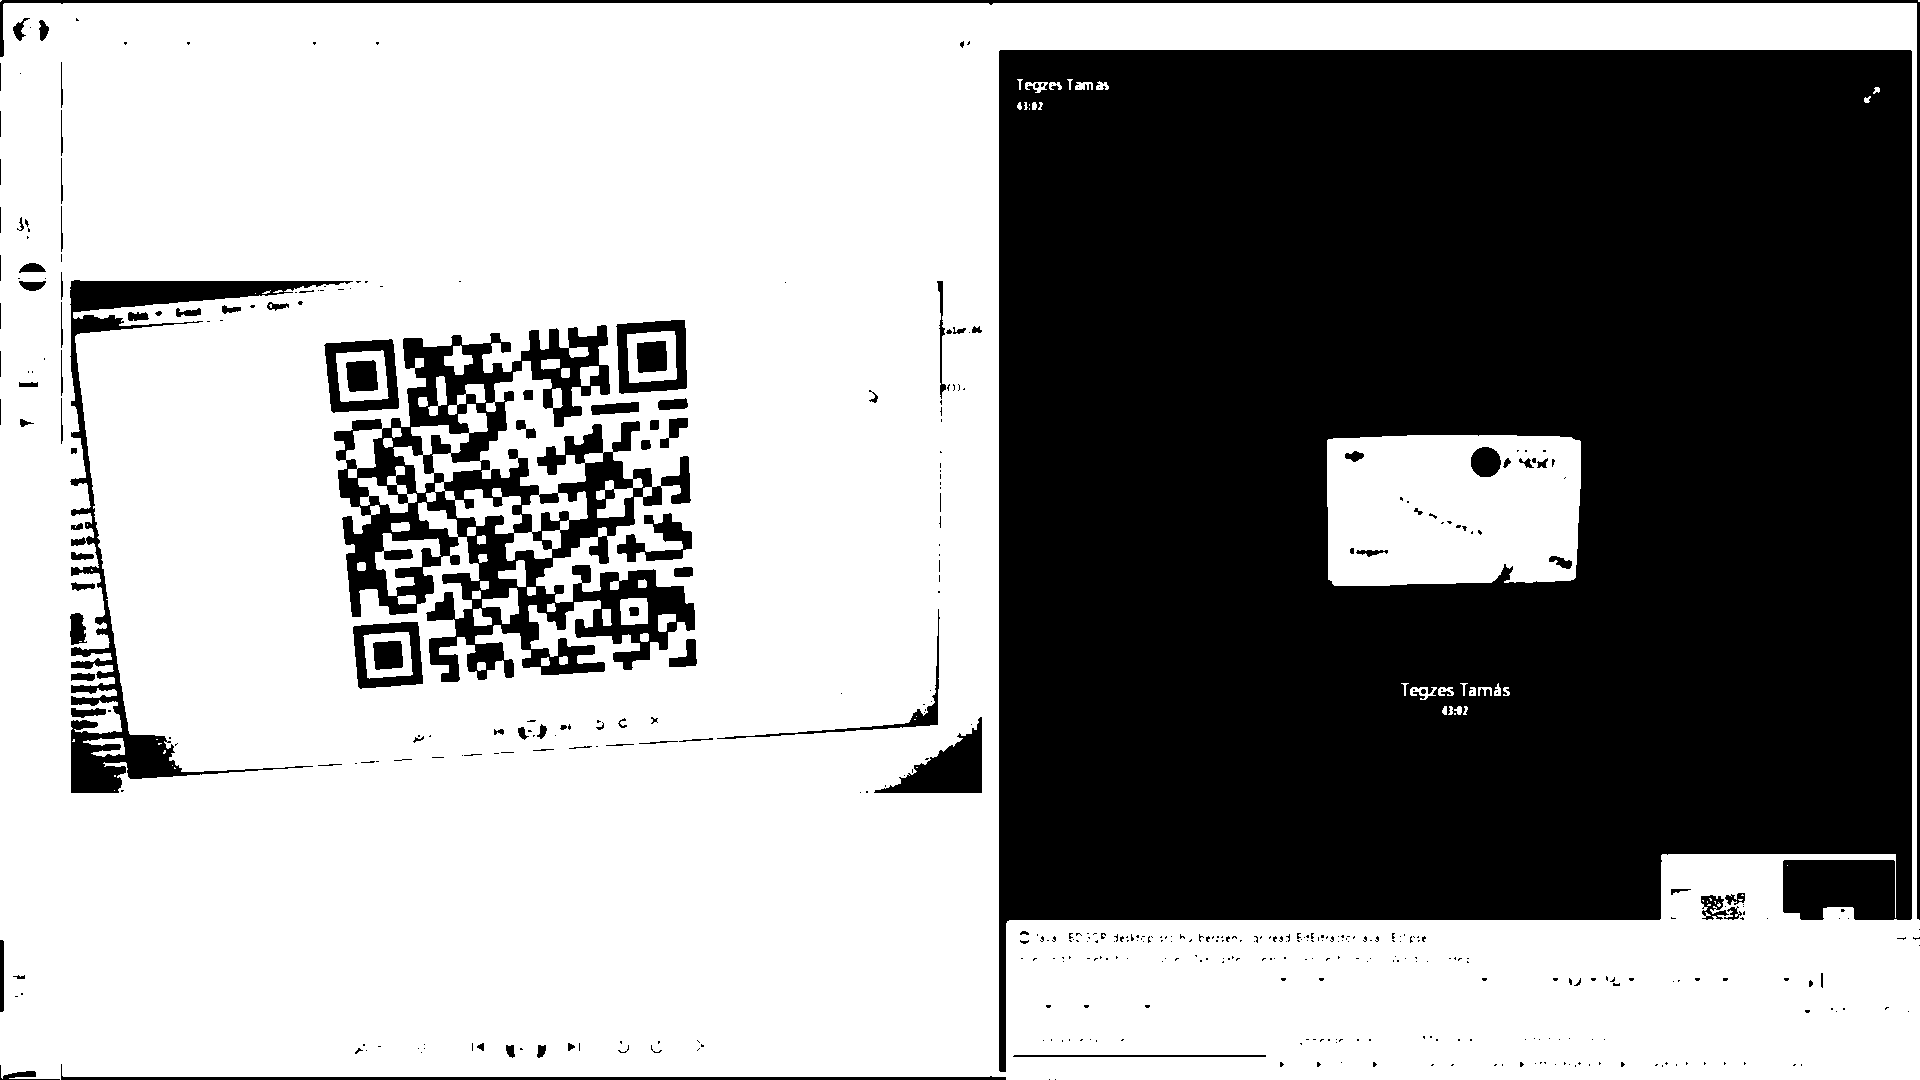
\includegraphics[height=0.75\textheight]{bitmap.png}
\end{frame}

\begin{frame}{Alakzatok �s mintav�telez�s}
\centering
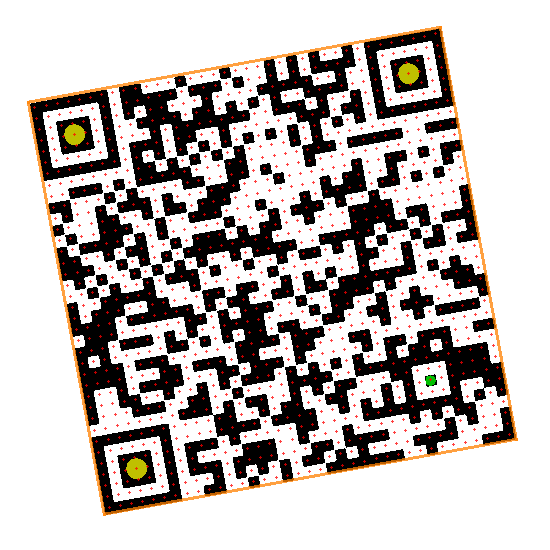
\includegraphics[height=0.75\textheight]{marked.png}
\end{frame}

\begin{frame}{Adatok}
\centering

\includegraphics[height=0.75\textheight]{qr0.png}
\end{frame}

\end{document}